Debido a la tarea de creación de datasets es muy tedioso, sobre todo por la tarea de etiquetado, aparte de buscar en Internet datasets realizados por terceros, podemos utilizar una herramienta que nos permite moldear uno a nuestro gusto. Esta herramienta se llama \textbf{OIDv4_ToolKit} \url{https://github.com/EscVM/OIDv4_ToolKit.git} y se encuentra en la cuarta carpeta \textit{4_Crear_Dataset}.\\

En el propio \textit{README.md} de la herramienta se nos explica su funcionamiento, si por ejemplo quisiéramos descargar un dataset que estuviera formado por 8 imágenes de coches y autobuses podríamos hacer:

\begin{lstlisting}
python3 main.py downloader --classes Car Bus --type_csv train --multiclasses 1 --limit 8
\end{lstlisting}

En la figura \ref{dataset} podemos observar como en la carpeta \textit{OID/Dataset/train/Car_Bus/} se nos han descargado las 8 imágenes, incluyendo sus ficheros TXT con la información de etiquetado en el interior de la carpeta \textit{Label}:

\begin{figure}[H]
	\centering
	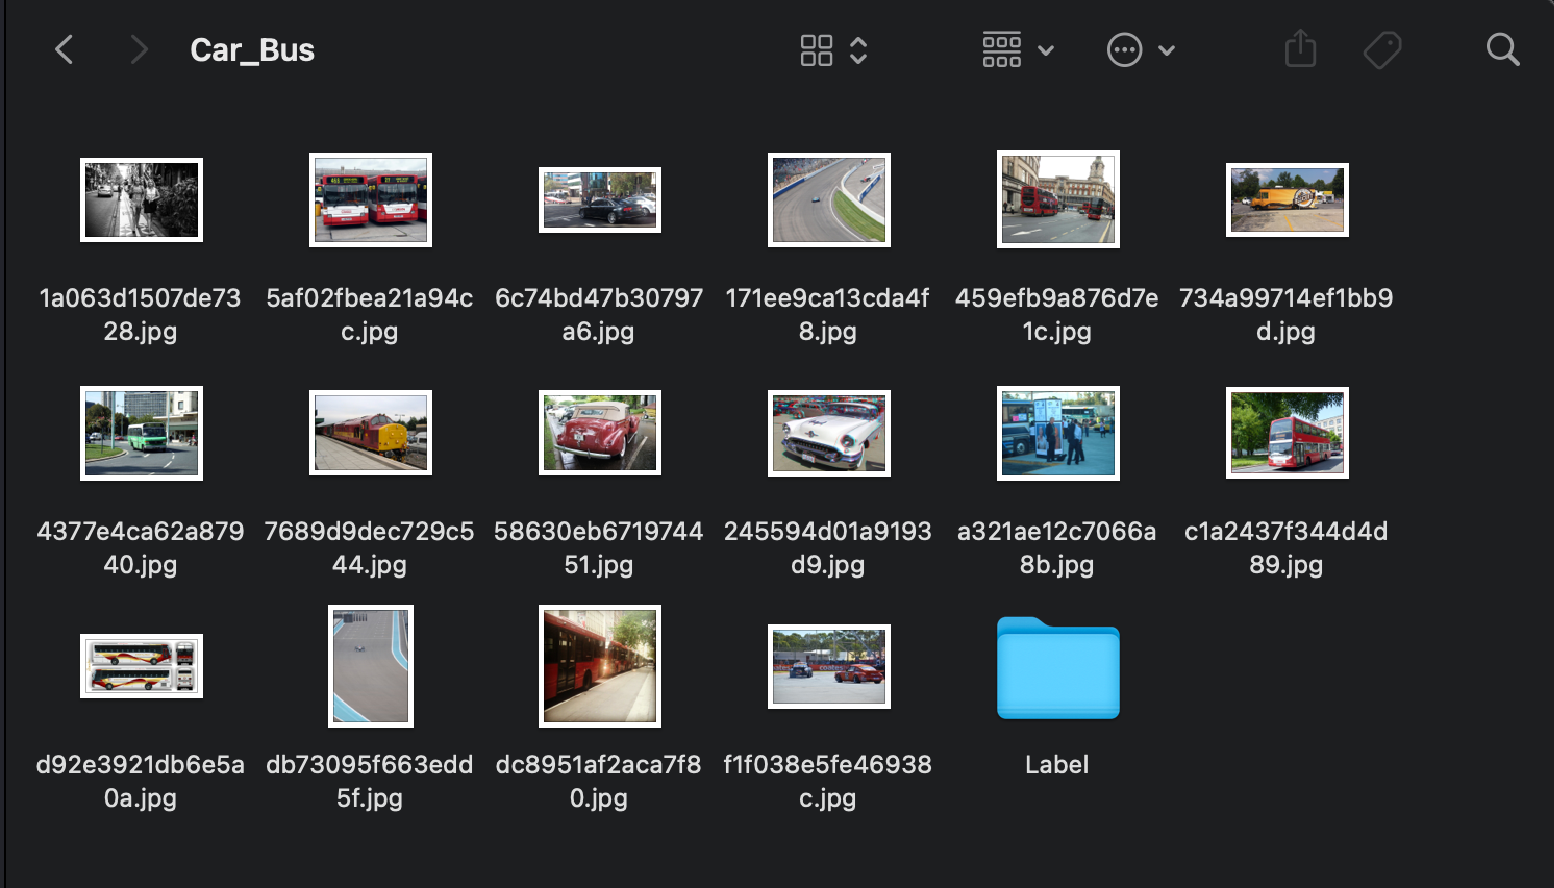
\includegraphics[width=\textwidth]{Imagenes/AnexoI_Manual/AA/dataset.pdf}
	\caption{Dataset descargado con los ficheros TXT}
	\label{dataset}
\end{figure}

Sin embargo, dichos ficheros con la información de etiquetado no se encuentran en formato \textbf{YOLO}, por lo que habrá que realizar la transformación. Dicha tarea se puede llevar a cabo mediante el script que se encuentra dentro de la herramienta \textbf{OIDv4_ToolKit} llamado \textbf{convert_to_YOLO.py}. \\

En dicho \textit{script} debemos cambiar introducir dos rutas, la que contiene las imágenes descargadas y en la que se encuentra el fichero CSV con todas las clases disponibles para descargar en la herramienta. Para obtener dichas rutas se pueden con un \textit{script} tan sencillo como este:

\begin{lstlisting}
import os
current_dir = os.path.dirname(os.path.abspath(__file__))
print(current_dir)
\end{lstlisting}

Tras ejecutar el \textit{script} podremos observar como en el directorio en el que se encuentran las imágenes se han creado cada uno de los ficheros TXT con el mismo nombre con la información de etiquetado \textbf{YOLO}. Podríamos comprobar además si se ha realizado con éxito la transformación abriendo dicho directorio con la herramienta de etiquetado \textbf{LabelImg}.
